\section{Functional Verification Experimental Results}
\label{eval}



% \subsection{Anomalies}
We evaluate the \emph{search} performance of SBS using the traces from the Eng. Bldg 2 and Cory Hall.
%% Romain
Due to the lack of historical data, such as room schedule or reports of energy waste, the evaluation is non-trivial.
Furthermore, getting ground truth data from a manual inspection of the hundreds traces of our data sets is impractical.
The lack of ground truth data prevents us from producing a systematic analysis of the anomalies missed by SBS (i.e. false negatives rate).
Nevertheless, we exhibit the relevance of the anomalies uncovered by SBS (i.e. high true positive rate and low false positive rate) by manually checking the output of SBS.
%% Romain

\paragraph{Anomaly classification}
To validate SBS results we manually inspect the anomalies detected by the algorithm.  
For each reported alarm $(t,i)$ we investigate the device trace $i$ and the devices correlated to it
to determine the reason for the alarm.
Specifically, we retrieve the major relationship change that causes the alarm (i.e. $\max(|w_j(C_{i,j}^t - R_{i,j})|)$, 
see Section \ref{methodo:ano}) and examine the metadata associated to the corresponding device.
% $j$ and the sign of the relationship change $C_{i,j}^t - R_{i,j}$.
% A positive value of relation change means the devices correlation at the time bin $t$ is abnormally high, whereas negative value means that the relationship between the two devices is broken.
This investigation allows us to classify the alarms into five groups:
\begin{itemize}
 \item \emph{High power usage}: alarms corresponding to electricity waste.
 \item \emph{Low power usage}: alarms representing the abnormally low electricity consumption of a device.
 \item \emph{Punctual abnormal usage}: alarms standing for short term (less than 2.5 hours) raise or drop of the electricity consumption.
 \item \emph{Missing data}: alarms raised due to a sensor failure.
 \item \emph{Other}: alarms whose root cause is unclear.
\end{itemize}

% However, the exhaustive enumeration of the true negatives (i.e. saving opportunities that are not detected) is impractical because of the size of the analyzed datasets (number of devices and traces length).
% Instead we exhibit the detector sensitivity by varying $\tau$, the threshold value.

\begin{figure}
\begin{center}
 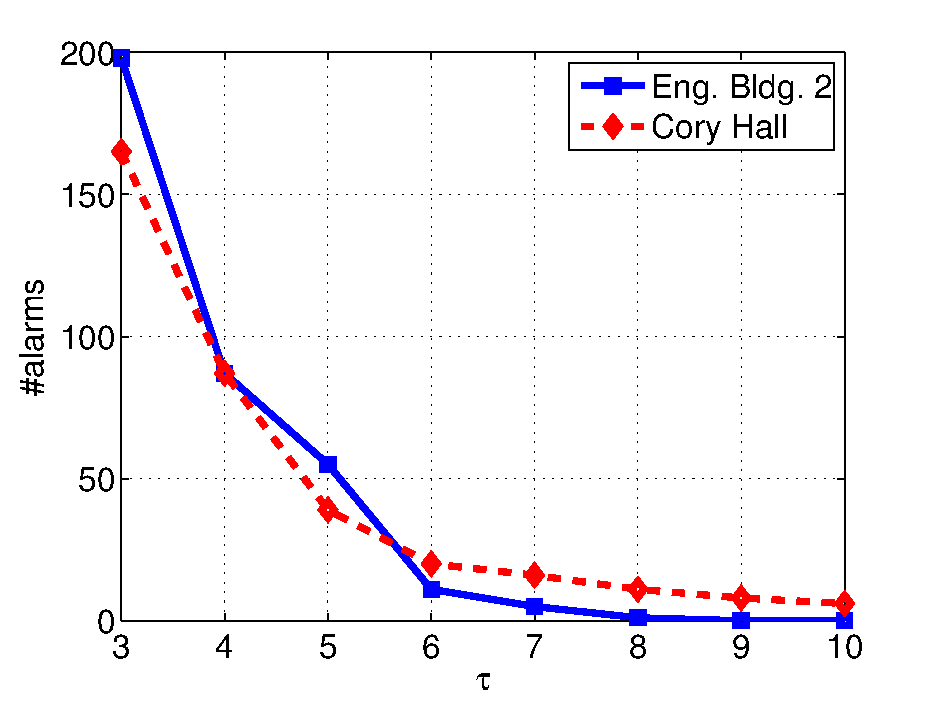
\includegraphics[width=.49\textwidth]{figs/threshold-eps-converted-to.pdf}
 \caption{Number of reported alarms for various threshold value ($\tau=[3,10]$).}
 \label{fig:thres}
 \end{center}
\end{figure}

\begin{table}
\begin{center}
\begin{tabular}{|l||c|c|c|c|c|}
\hline
&High&Low&Punc.&Missing&Other\\ \hline \hline
Eng. Bldg 2 & 9 (5) & 6 (5) & 1 (1) & 36 (1) & 3 (3) \\ \hline
Cory Hall & 25 (7) & 7 (3) & 4 (4) & 0 (0) & 3 (3) \\ \hline
\end{tabular}
\end{center}
\caption{Classification of the alarms reported by SBS for both dataset (and the number of corresponding anomalies).}
\label{tab:classif}
\end{table}

\paragraph{Experimental setup}
For each experiment, the data is split in time bins of one day, starting from 09:00 a.m. -- which is approximately 
the office's opening time.
We avoid having bins start at midnight since numerous anomalies appear at night and they are better highlighted if they are 
not spanning two time bins.
Only the data at medium frequencies are analyzed, the other frequency bands are ignored, and the reference matrix is computed from all time bins.


The threshold $\tau$ tunes the sensitivity of SBS, hence, the number of reported alarms.  
Furthermore, by plotting the number of alarms against the value of $\tau$ for both datasets (Figure \ref{fig:thres}) we observe an 
elbow in the graph around $\tau=5$.
With thresholds lower than this pivot value ($\tau<5$), the number of alarms significantly increases, causing less important anomalies 
to be reported.  
For higher values ($\tau>5$), the number of alarms is slowly decreasing, providing more conservative results that consist of the 
most important anomalies.
This pivot value provides a good trade off for either data set.

\begin{figure*}
  \subfloat[High power usage where the HVAC (EHP) is turned on at night\label{fig:res:eng1}]{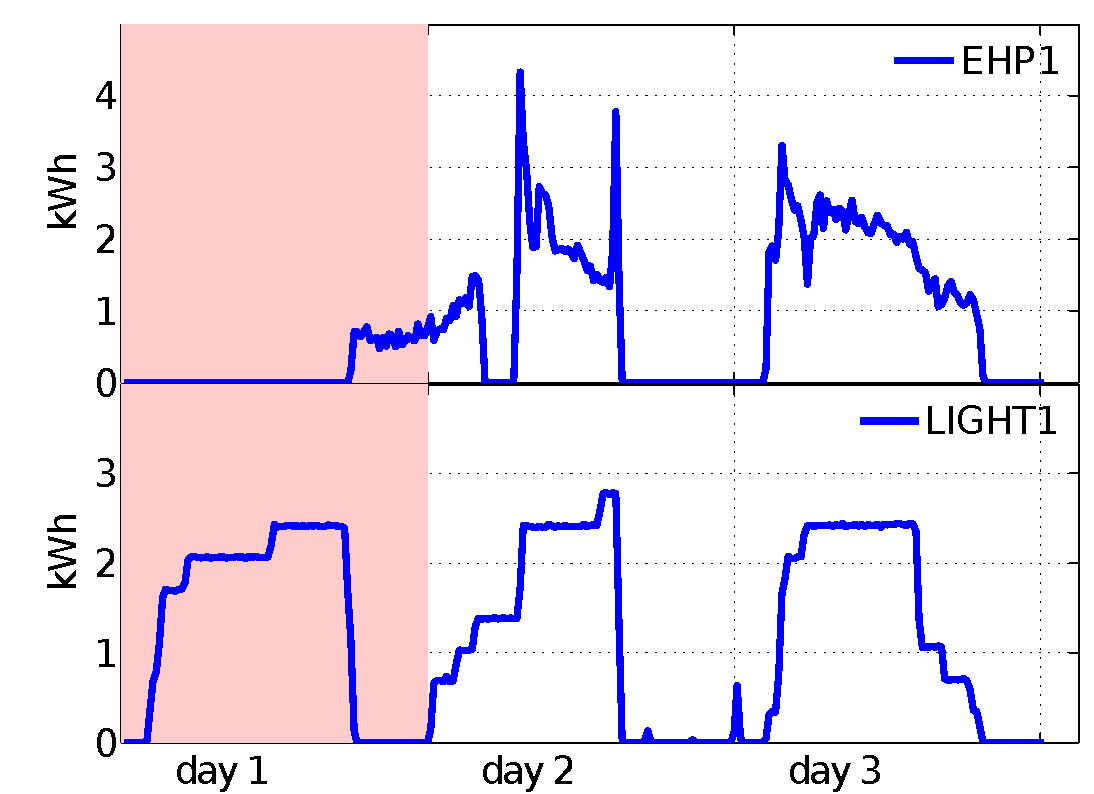
\includegraphics[width=.32\textwidth]{figs/0sig20_sig31alarm1-eps-converted-to.pdf}} \hspace{.015\textwidth} %EHP turned on at night!?
  \subfloat[High power usage where the light is left on at night\label{fig:res:eng2}]{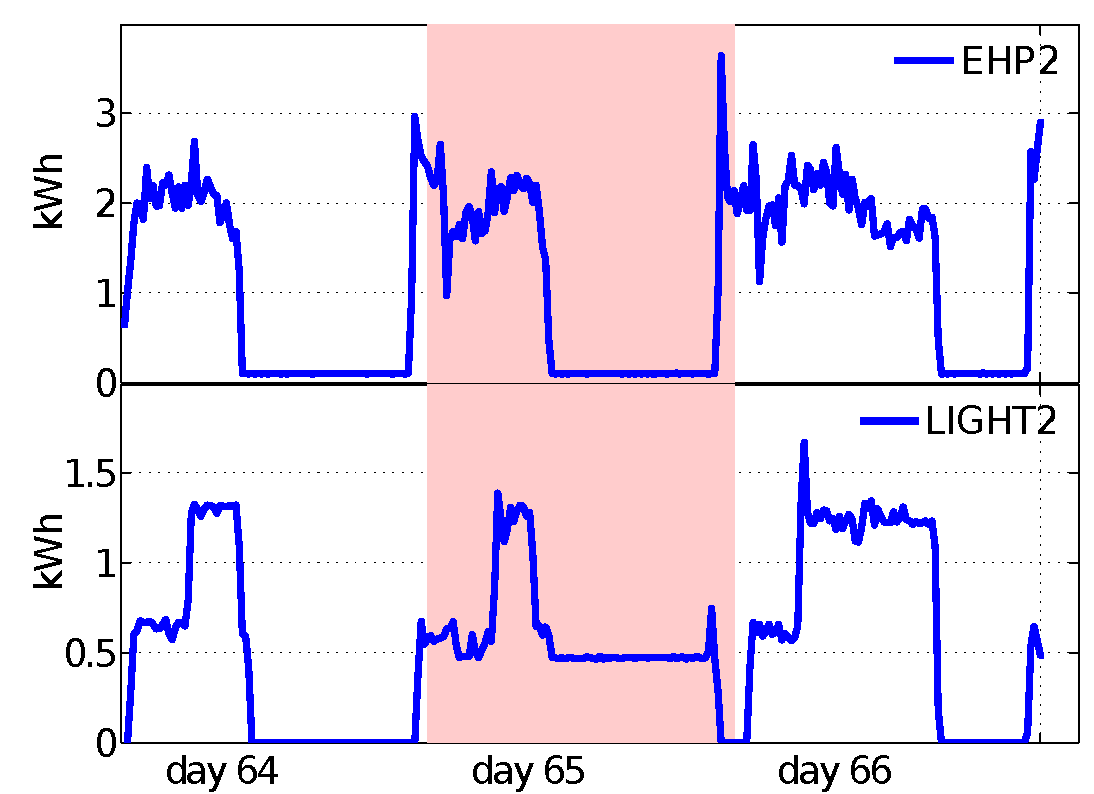
\includegraphics[width=.32\textwidth]{figs/0sig123_sig134alarm65-eps-converted-to.pdf}} \hspace{.015\textwidth}  %Light left on during night
 \subfloat[Low power usage where the HVAC (EHP) is not used during office hours\label{fig:res:eng3}]{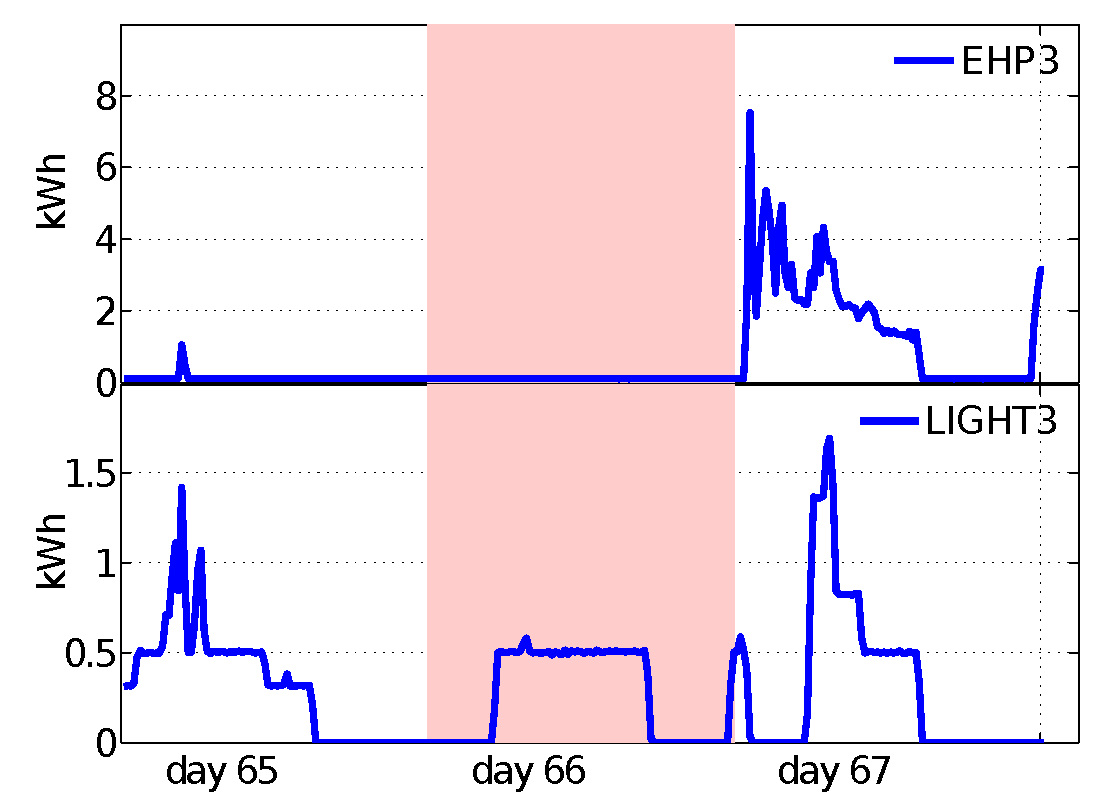
\includegraphics[width=.32\textwidth]{figs/0sig24_sig33alarm66-eps-converted-to.pdf}}\\ %Three EHPs that are really correlated
 \subfloat[Long term high power usage partially detected\label{fig:res:eng4}]{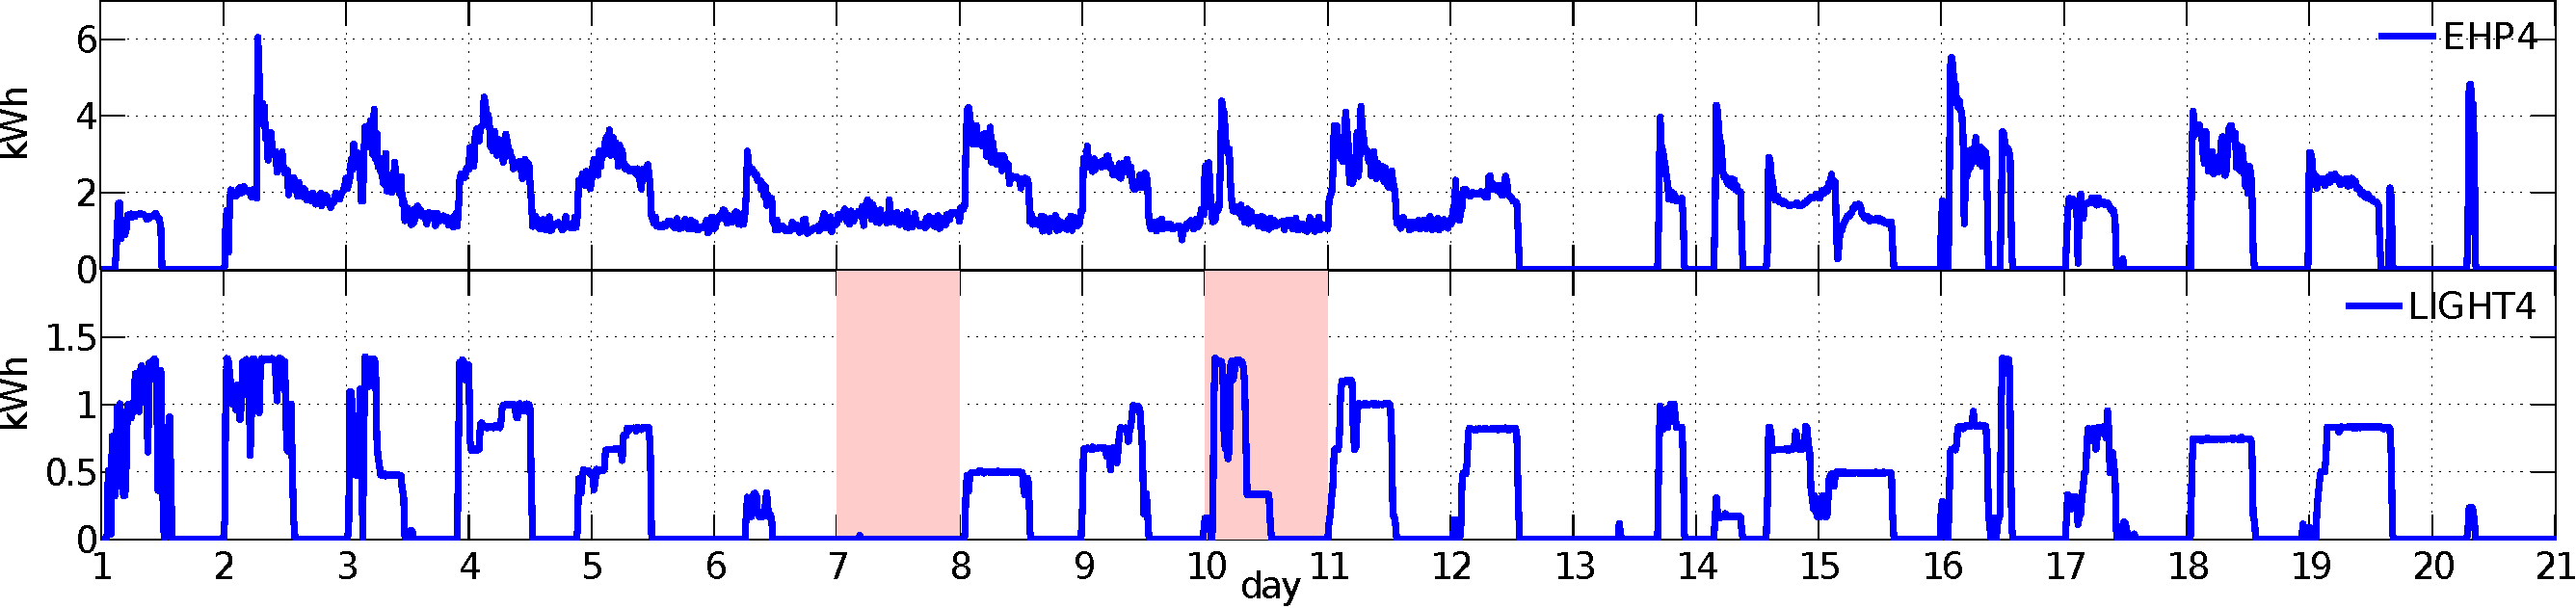
\includegraphics[width=\textwidth]{figs/0sig3_sig15alarm7-eps-converted-to.pdf}}\\  
\caption{Example of alarms (red rectangles) reported by SBS on the Eng. Bldg 2 dataset}
\end{figure*}


Table \ref{tab:classif} classifies the alarms reported by SBS on both datasets.
 Anomalies spanning several time bins (or involving several devices) may raise several alarms.  We display these in Table \ref{tab:classif} 
 as numbers in brackets -- the number of anomalies corresponding to the reported alarms.
%Due to page limitation the following sections only present the most typical and interesting anomalies identified by SBS.

\subsection{Alarms in Todai}


SBS reported 55 alarms over the 10 weeks of the Eng. Bldg 2 dataset.
However, 36 alarms are set aside because of sensor errors; one GHP has missing data for the first 18 days.
Since this device is highly correlated to the GHP in the reference matrix, their relationship is broken for the 18 first bins and 
for each bin one alarm per device is raised.

\begin{figure*}
  \subfloat[Low power usage due to a chiller failure\label{fig:res:cory1}]{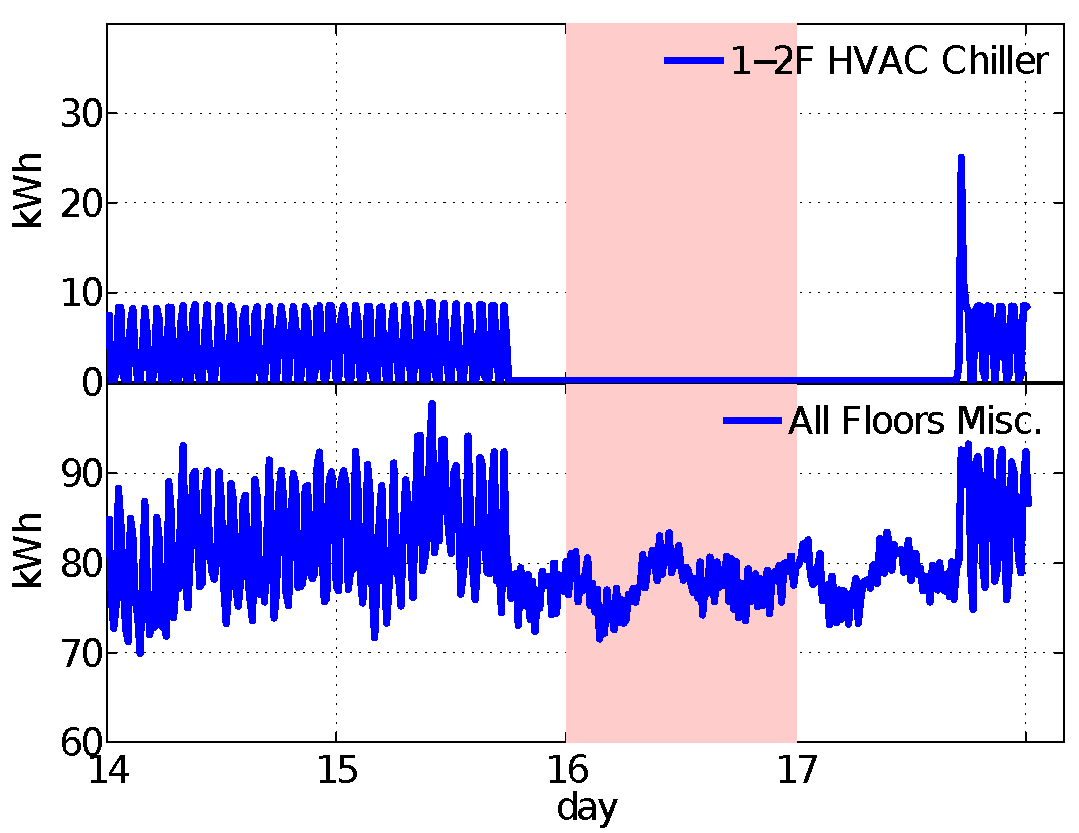
\includegraphics[width=.32\textwidth]{figs/1sig37_sig55alarm16-eps-converted-to.pdf}} \hspace{.015\textwidth}
 \subfloat[High power usage highlighted by the elevator usage\label{fig:res:cory21}]{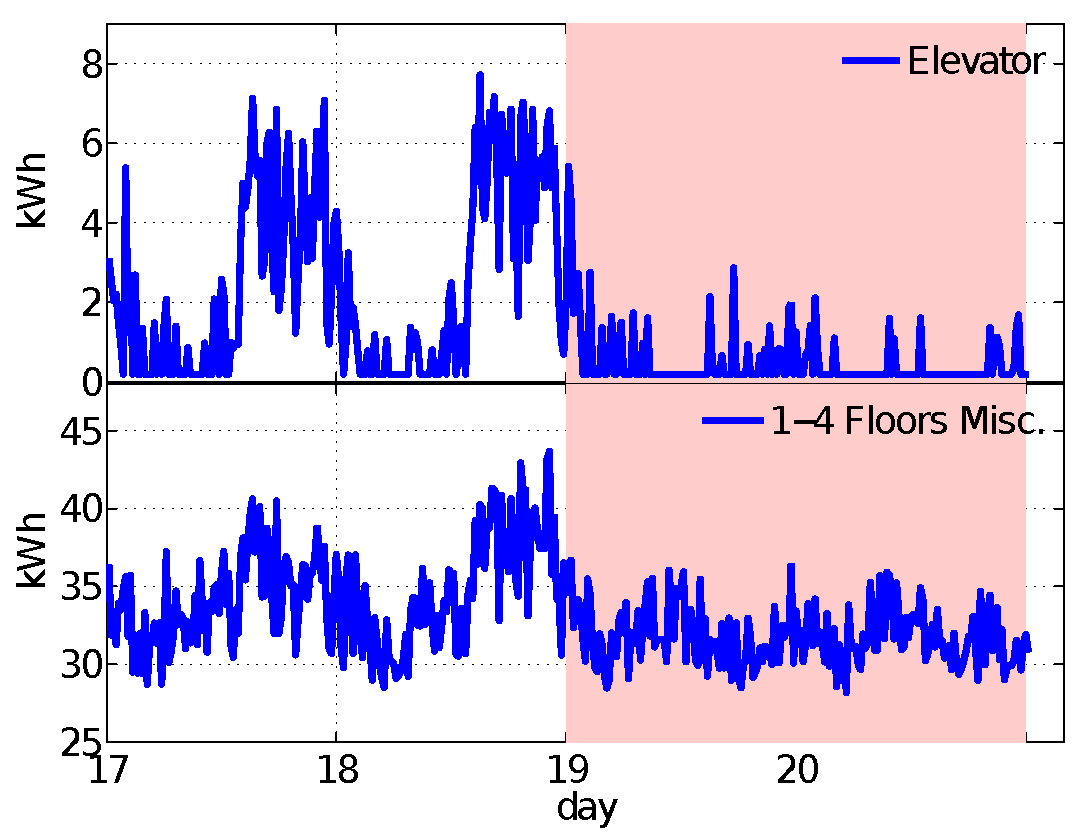
\includegraphics[width=.32\textwidth]{figs/1sig7_sig49alarm19-eps-converted-to.pdf}}
 \hspace{.015\textwidth}
 \subfloat[Normal power and elevator usage\label{fig:res:cory22}]{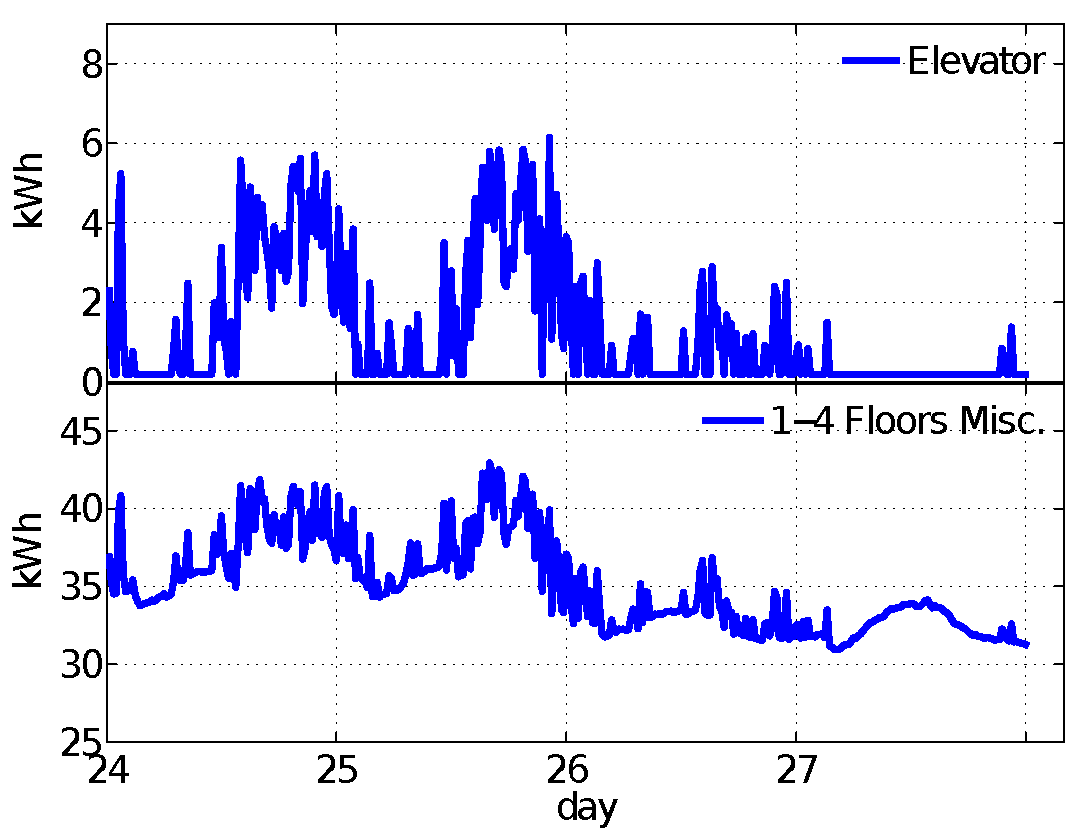
\includegraphics[width=.32\textwidth]{figs/1sig7_sig49alarm-eps-converted-to.pdf}}\\ 
 \subfloat[Long term high power usage due to competing heating and cooling\label{fig:res:cory3}]{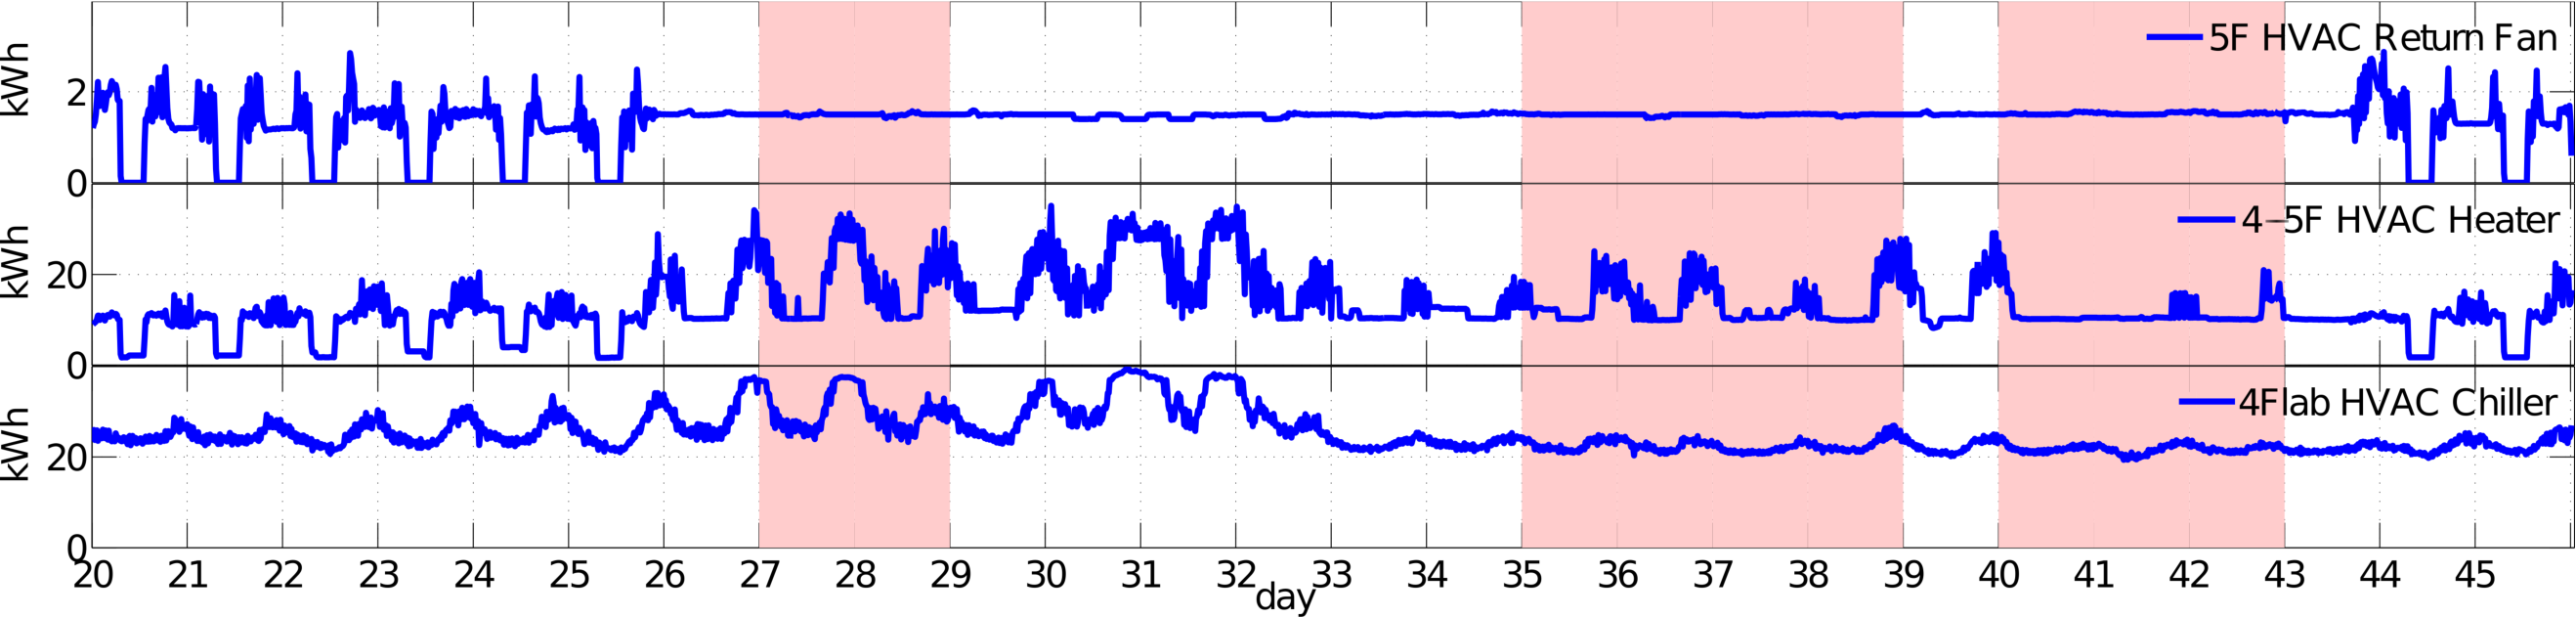
\includegraphics[width=\textwidth]{figs/1sig34_sig54alarm27-eps-converted-to.pdf}} 
\caption{Example of alarms (red rectangles) reported by SBS on the Cory Hall dataset}
\end{figure*}

In spite of the post-Fukushima measures to reduce Eng. Bldg 2's energy consumption, 
SBS reported nine alarms corresponding to high power usage (Table \ref{tab:classif}).
Figure \ref{fig:res:eng1} depicts the electricity consumption of the light and EHP in the same room where two alarms are raised.
Because the EHP was not used during daytime (but is turned on at night, when the light is turned off) the relationship between the two devices 
is ``broken'' and an alarm is raised for each device.
Figure \ref{fig:res:eng2} shows another example of energy waste.  The light is on at night and the EHP is off.
The top-priority anomaly reported by SBS is caused by the 10 days long constant use of an EHP (Figure \ref{fig:res:eng4}) and this 
waste of electricity accounts for 165 kWh.
SBS partially reports this anomaly but lower values of $\tau$ permits us to identify most of it.


We observed six alarms corresponding to abnormally low power use.  Upon further inspection we notice that it corresponds to energy saving
 initiatives from the occupants -- likely due to electricity concerns in Japan.
This behavior is displayed in Figure \ref{fig:res:eng3}.  The room is occupied at the usual office hours (indicated by light usage)  but the 
EHP is not on in order to save electricity.

\subsection{Alarms in Cory Hall}
SBS reported 39 alarms for the Cory Hall dataset (Table \ref{tab:classif}).
 Seven are classified as low power usage, however, our inspection revealed that the root causes are different than for the Eng. Bldg 2 dataset.
We observe that the low power usage usually corresponds to device failures or misconfiguration.  
For example, Figure \ref{fig:res:cory1} depicts the electricity consumption of the $2^{nd}$ floor chiller and a power riser that comprises the consumption of multiple systems, including the chiller.
As the chiller suddenly stops working, the correlation between both measurements is significantly altered and an alarm for each device is raised.

SBS also reports 25 alarms corresponding to high power usage. 
One of the identified anomalies is particularly interesting.
We indirectly observe abnormal usage of a device from the power consumption of the elevator and a power panel for equipment from 
the $1^{st}$ to the $4^{th}$ floor.
Figure~\ref{fig:res:cory21} and~\ref{fig:res:cory22} show the electricity consumption for both devices. 
SBS uncovers the correlation between the these two signals, as the amount of electricity going through the panel fluctuates along with the elevator power consumption (Figure \ref{fig:res:cory22}).
In fact, the elevator is a good indicator of the building's occupancy.
Anomalous energy-consumption is identified during a weekend as the consumption measured at the panel is independently fluctuating from the elevator usage.
These fluctuations are caused by a device that is not directly monitored.  Therefore, we could not identify the root cause more precisely. 
 Nevertheless, the alarm is worthwhile for building operators to start investigating.

The most important anomaly identified in Cory Hall is shown in Figure \ref{fig:res:cory3}.
This anomaly corresponds to the malfunctioning of the HVAC heater serving the $4^{th}$ and $5^{th}$ floors. 
The heater is constantly working for 18 consecutive days, regardless of the underlying occupant activity.
Moreover, in order to maintain appropriate temperature this also results in an increase of the $4^{th}$ floor HVAC chiller power consumption 
and several fans, such as the one depicted in Figure \ref{fig:res:cory3}.
This situation is indicative of simultaneous heating and cooling -- whereby heating and cooling systems are competing -- and it 
is a well-know problem in building management that leads to significant energy waste.
For this example, the electricity waste is estimated around 2500 kWh for the heater.
Nevertheless, as the anomaly spans over 18 days, it is hidden in the building's overall consumption, thus, it is difficult to detect 
by building administrators without SBS.
